\documentclass{article}

\usepackage{graphicx}
\usepackage{amsmath}
\usepackage{bm}
\usepackage{appendix}
\usepackage{float}

\begin{document}

\title{\vspace{1cm}Project 1 \\ FYS3150}

\author{\vspace{1cm}Ann-Silje Kirkvik \\ github.com/annsilje/fys3150}
\date{\vspace{5cm}\today}

\maketitle

\newpage

\begin{abstract}
This project investigates different numerical methods for solving linear second order differential equations of a certain form. The second order derivative is approximated numerically and yields a linear equation system with a sparse matrix. Three methods are tested for this specific problem. One is a full scale LU-decomposition and backward substitution that also works on dense matrices. The other two methods utilize the fact that the matrix is tridiagonal and has constant values for the diagonals. As expected the fastest algorithm is the one specifically tailored to the second order derivative approximation. 
\end{abstract}

\vspace{1cm}

%describe problem (short)
\section{Introduction}
This project will explore different numerical methods for solving linear second order differential equations of the form

\begin{equation}
\label{eq:diff_eq}
-u''(x) = f(x), x \in(0,1), u(0) = u(1) = 0.
\end{equation}

This problem can be rewritten into a set of linear equation $\bm{A}\bm{x}=\bm{b}$ with the nice property that the matrix $\bm{A}$ is tridiagonal. This particular matrix even has an analytical solution, which enables the creation of a tailored algorithm that is fast and memory efficient compared to a brute force linear equation solver. Section \ref{sec:description} explains the theoretical background for the different numerical algorithms tested in this project. Section \ref{sec:results} contains the results for the tests performed and section \ref{sec:conclusions} has some concluding remarks.

%describe theory
\section{Description}
\label{sec:description}
Starting with a Taylor expansion of $u(x_i + h) = u_{i+1}$ and $u(x_i - h)= u_{i-1}$ and adding these together yields the three point formula, from chapter 3.1 in \cite{lectures}, for the second order derivative:

\begin{equation*}
u''(x) = \frac{u_{i+1} + u_{i-1} - 2u_i}{h^2} + \mathcal{O}(h^2).
\end{equation*}

The numerical approximation $v''_i(x_i)$ to $u''(x)$ is then
  
\begin{equation*}
v''_i(x_i) = \frac{v_{i+1} + v_{i-1} - 2v_i}{h^2}.
\end{equation*}

Inserting this approximation into the original differential equation in \ref{eq:diff_eq} yields the following formula:

\begin{equation*}
-\frac{v_{i+1} + v_{i-1} - 2v_i}{h^2} = f_i,
\end{equation*}

for a given set of grid points $(x_i, f_i(x_i))$ for $i=1,...,n$, where $h=1/(n+1)$ is the step length between each $x_i$. With the boundary conditions $v_0 = v_{n+1} = 0$ this becomes $n$ linear equations:

\begin{flalign*}
2v_1 - v_2 &= h^2f_1 \\
-v_1 + 2v_2 - v_3 &= h^2f_2 \\
-v_2 + 2v_3 - v_4 &= h^2f_3 \\
&\vdots \\
-v_{n-1} + 2v_n - v_{n+1} &= h^2f_n \\
\end{flalign*} 

In matrix form this becomes $\bm{A}\bm{v} = h^2\bm{f}$ or 

\begin{equation*}
\begin{bmatrix}
2      & -1     & 0       & \cdots  & \cdots  & \cdots  & 0      \\
-1     & 2      & -1      & 0       & \cdots  & \cdots  & 0      \\
0      & -1     & 2       & -1      & 0       & \cdots  & 0      \\
\vdots & \vdots & \ddots  & \ddots  & \ddots  & \vdots  & \vdots \\
\vdots & \vdots & \vdots  & \ddots  & \ddots  & \ddots  & \vdots \\
0      & \cdots & \cdots  & 0       & -1      & 2       & -1     \\
0      & \cdots & \cdots  & \cdots  & 0       & -1      & 2      \\
\end{bmatrix}
\begin{bmatrix}
v_1 \\
v_2 \\
v_3 \\
\vdots \\
\vdots \\
v_{n-1} \\
v_n \\
\end{bmatrix}
= h^2
\begin{bmatrix}
f_1 \\
f_2 \\
f_3 \\
\vdots \\
\vdots \\
f_{n-1} \\
f_n \\
\end{bmatrix}
\end{equation*}

This linear equation system can be solved numerically in at least three different ways:

\begin{itemize}
\item By LU-decomposition and backward substitution.
\item With a tridiagonal solver and backward substitution.
\item With a analytical custom made solver and backward substitution.
\end{itemize}

\subsection{LU-decomposition}
LU-decomposition consists of finding a factorization $\bm{A}=\bm{L}\bm{U}$ such that $\bm{L}$ is a lower triangular matrix and $\bm{U}$ is an upper triangular matrix. For instance if $\bm{A}$ is a $4 \times 4$ matrix one such factorization is:

\begin{equation*}
\bm{L}=
\begin{bmatrix}
1      & 0      & 0       & 0       \\
l_{21} & 1      & 0       & 0       \\
l_{31} & l_{32} & 1       & 0       \\
l_{41} & l_{42} & l_{43}  & 1       \\
\end{bmatrix}
\quad \text{ and } \quad
\bm{U}=
\begin{bmatrix}
u_{11} & u_{12} & u_{13} & u_{14}   \\
0      & u_{22} & u_{23} & u_{24}   \\
0      & 0      & u_{33} & u_{34}   \\
0      & 0      & 0      & u_{44}   \\
\end{bmatrix}
\end{equation*}

Once this factorization is found the equation system $\bm{A}\bm{v}=\bm{L}\bm{U}\bm{v}=h^2\bm{f}$ can be solved by setting $\bm{L}\bm{y}=h^2\bm{f}$ and $\bm{U}\bm{v}=\bm{y}$ and applying backward substitution twice. This execution time of this algorithm scales as $\mathcal{O}(n^3)$ as described in appendix \ref{app:lud}.   


\subsection{Tridiagonal solver}
A tridiagonal solver exploits the fact that only the diagonal elements and the elements directly above and below the diagonal are different from zero. The matrix $\bm{A}$ then has the form:

\begin{equation*}
\bm{A} = 
\begin{bmatrix}
b_1    & c_1    & 0       & \cdots  & \cdots  & \cdots  & 0      \\
a_2    & b_2    & c_2     & 0       & \cdots  & \cdots  & 0      \\
0      & a_3    & b_3     & c_3     & 0       & \cdots  & 0      \\
\vdots & \vdots & \ddots  & \ddots  & \ddots  & \vdots  & \vdots \\
\vdots & \vdots & \vdots  & \ddots  & \ddots  & \ddots  & \vdots \\
0      & \cdots & \cdots  & 0       &a_{n-1} & b_{n-1} & c_{n-1} \\
0      & \cdots & \cdots  & \cdots  & 0       & a_n     & b_n    \\
\end{bmatrix}
\end{equation*}

By performing Gauss elimination on the equation system it can be shown that the elements directly above the diagonal remains unchanged and the diagonal elements $d_i$ become 

\begin{equation}
d_i = b_i - a_ic_{i-1}/d_{i-1} \qquad \text{ with } d_1 = b_1.
\label{eq:diag}
\end{equation}

The elements directly below the diagonal becomes zero, as is the goal of the Gauss elimination. The column vector elements $w_i$ becomes 

\begin{equation}
w_i = f_i - a_iw_{i-1}/d_{i-1} \qquad \text{ with } w_1 = f_1.
\label{eq:col}
\end{equation}

The detailed steps of the Gauss elimination are listed in appendix \ref{app:gauss}. The equation system can then finally be solved with backward substitution where 
\begin{equation}
v_i = w_{i-1} - c_{i-1}v_i/d_{i-1} \qquad \text{ with } v_n = h^2w_n/d_n.
\label{eq:back}
\end{equation}

Equation \ref{eq:diag} consists of three floating point operations which are then performed $n$ times. (Ignoring the fact that the first element is easier to find). The same applies for equation \ref{eq:col}. Finding the upper triangular equation system then requires $2*3n=6n$ floating point operations, which scales as $\mathcal{O}(n)$. The backward substitution also requires three floating point operations and therefore the algorithm as a whole scales as $\mathcal{O}(n)$. The factor $h^2$ is not a part of the generic tridiagonal solver, but rather a constant specific to the problem of approximating the second order derivative and is therefore not considered when counting floating point operations. 


\subsection{Custom solver}

The matrix $\bm{A}$ is not only tridiagonal but all the elements $a_i=-1$, $b_i=2$ and $c_i=-1$. Inserting this into equations \ref{eq:diag}, \ref{eq:col} and \ref{eq:back} respectively yields 

\begin{flalign*}
d_i &= 2 - 1/d_{i-1} \qquad \text{ with } d_1 = 2 \\
w_i &= f_i + w_{i-1}/d_{i-1} \qquad \text{ with } w_1 = f_1 \\
v_i &= w_{i-1}  + v_i/d_{i-1} \qquad \text{ with } v_n = h^2w_n/d_n \\
\end{flalign*}

Calculating the first few instances of $d_i$ reveals a pattern:

\begin{flalign*}
d_1 &= 2 \\
d_2 &= 2 - 1/2 = 3/2 \\
d_3 &= 2 - 1/(3/2) = 4/3 \\
d_4 &= 2 - 1/(4/3) = 5/4 \\
\vdots \\
d_i &= (i+1)/i.
\end{flalign*}

Having precalculated some of the floating point operations, this algorithm is even faster than the generic tridiagonal solver. Finding the diagonal requires one floating point operation per element, a total of $n$ floating point operations. Finding the new column vector is reduced to two floating point operations per element and the same with the backward substitution. This gives a total of $(2+1)n=3n$ floating point operations for finding the upper triangular equation system and $2n$ floating point operations for the backward substitution. As with the generic tridiagonal solver the algorithm scales as $\mathcal{O}(n)$.


%describe how the theory was applied to solve the problem (short)
\section{Results}
\label{sec:results}

If $f(x) = 100e^{-10x}$ the analytical solution to the differential equation in \ref{eq:diff_eq} is $u(x) = 1 - (1 - e^{-10})x - e^{-10x}$. Because the analytical solution is known the function $f(x)$ is useful for testing the numerical algorithms. The three solvers are tested for different values of $n$ and the source code is found on the project's github address https://github.com/annsilje/fys3150/.

\subsection{Precision}
Figure \ref{fig:g_vs_a} shows the difference between the analytical solution and the numerical solution using the generic tridiagonal solver for $n=10, 10^2,..10^7$. The endpoints are excluded in the plot. With shorter step lengths $h$ (higher $n$) the difference gets smaller and there does not seem to be any problems with loss of precision due to round of errors with the values that were tested. Similar plots for the custom made solver and the LU-decomposition solver is shown in figure \ref{fig:s_vs_a} and \ref{fig:lud_vs_a} in appendix \ref{app:diff_plots}. 

\begin{figure}[H]
    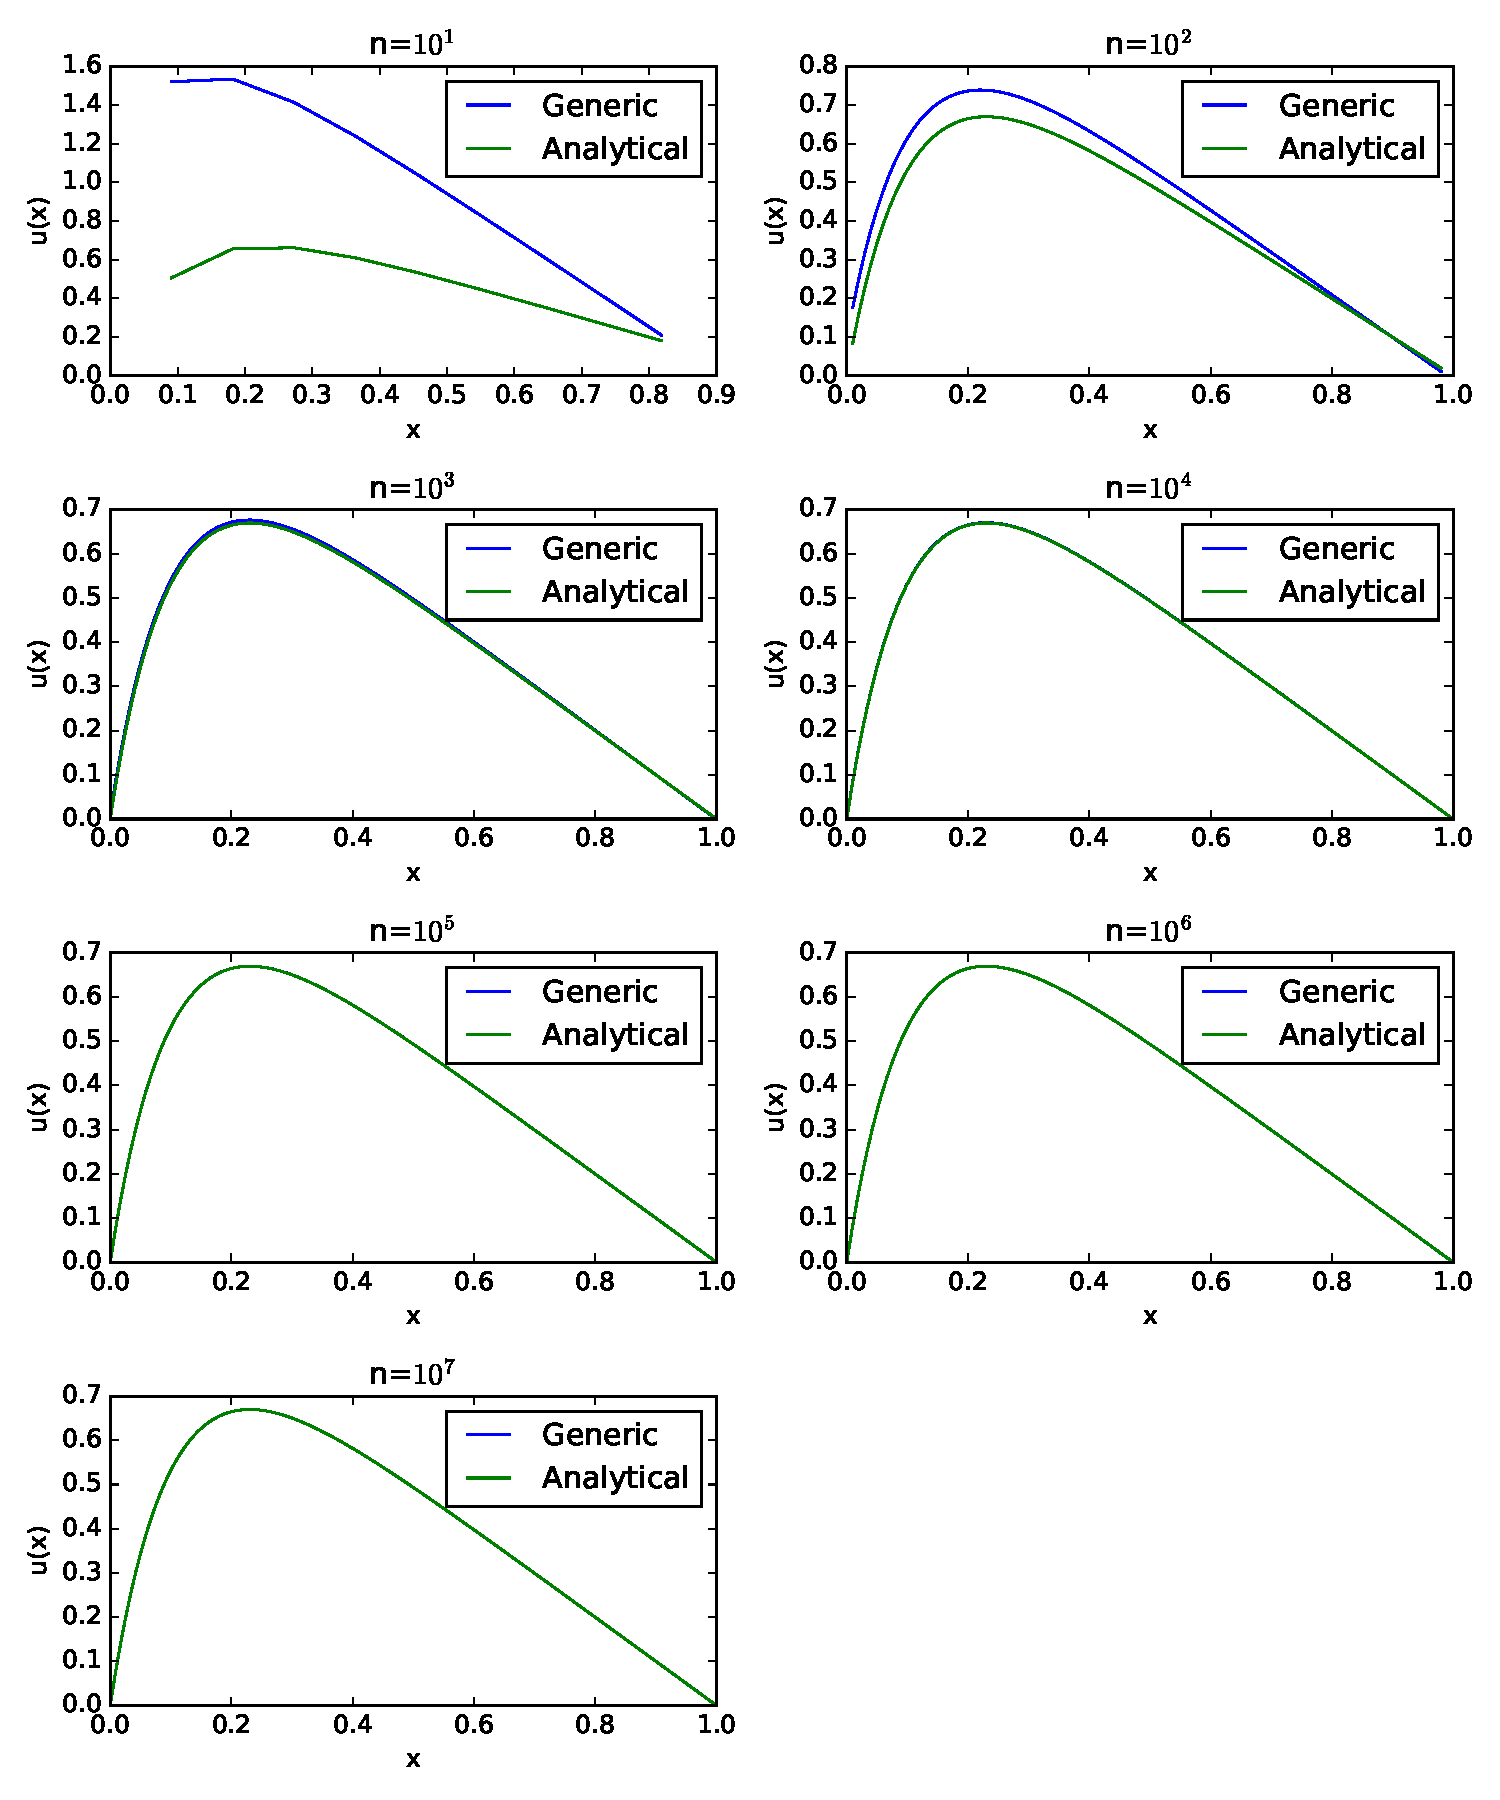
\includegraphics[width=\linewidth]{fig/generic_vs_analytical.pdf}
    \caption{Numerical solution using the generic tridiagonal solver compared to the analytical solution.}
    \label{fig:g_vs_a}
\end{figure}

The relative error of each step size is computed as 

\begin{equation}
\epsilon_i = \big|\frac{v_i - u_i}{u_i}\big|
\label{eq:error}
\end{equation}
and is plotted in figure \ref{fig:error}. The relative error seems to be close to zero for the middle region of $x \in (0,1)$, but as $x$ approaches the boundary conditions the error increases and reaches its maximum value at $x_1$. Since $u_i$ is approaching zero as $x \rightarrow 0$ and $x \rightarrow 1$, this seems reasonable. 

\begin{figure}[H]
    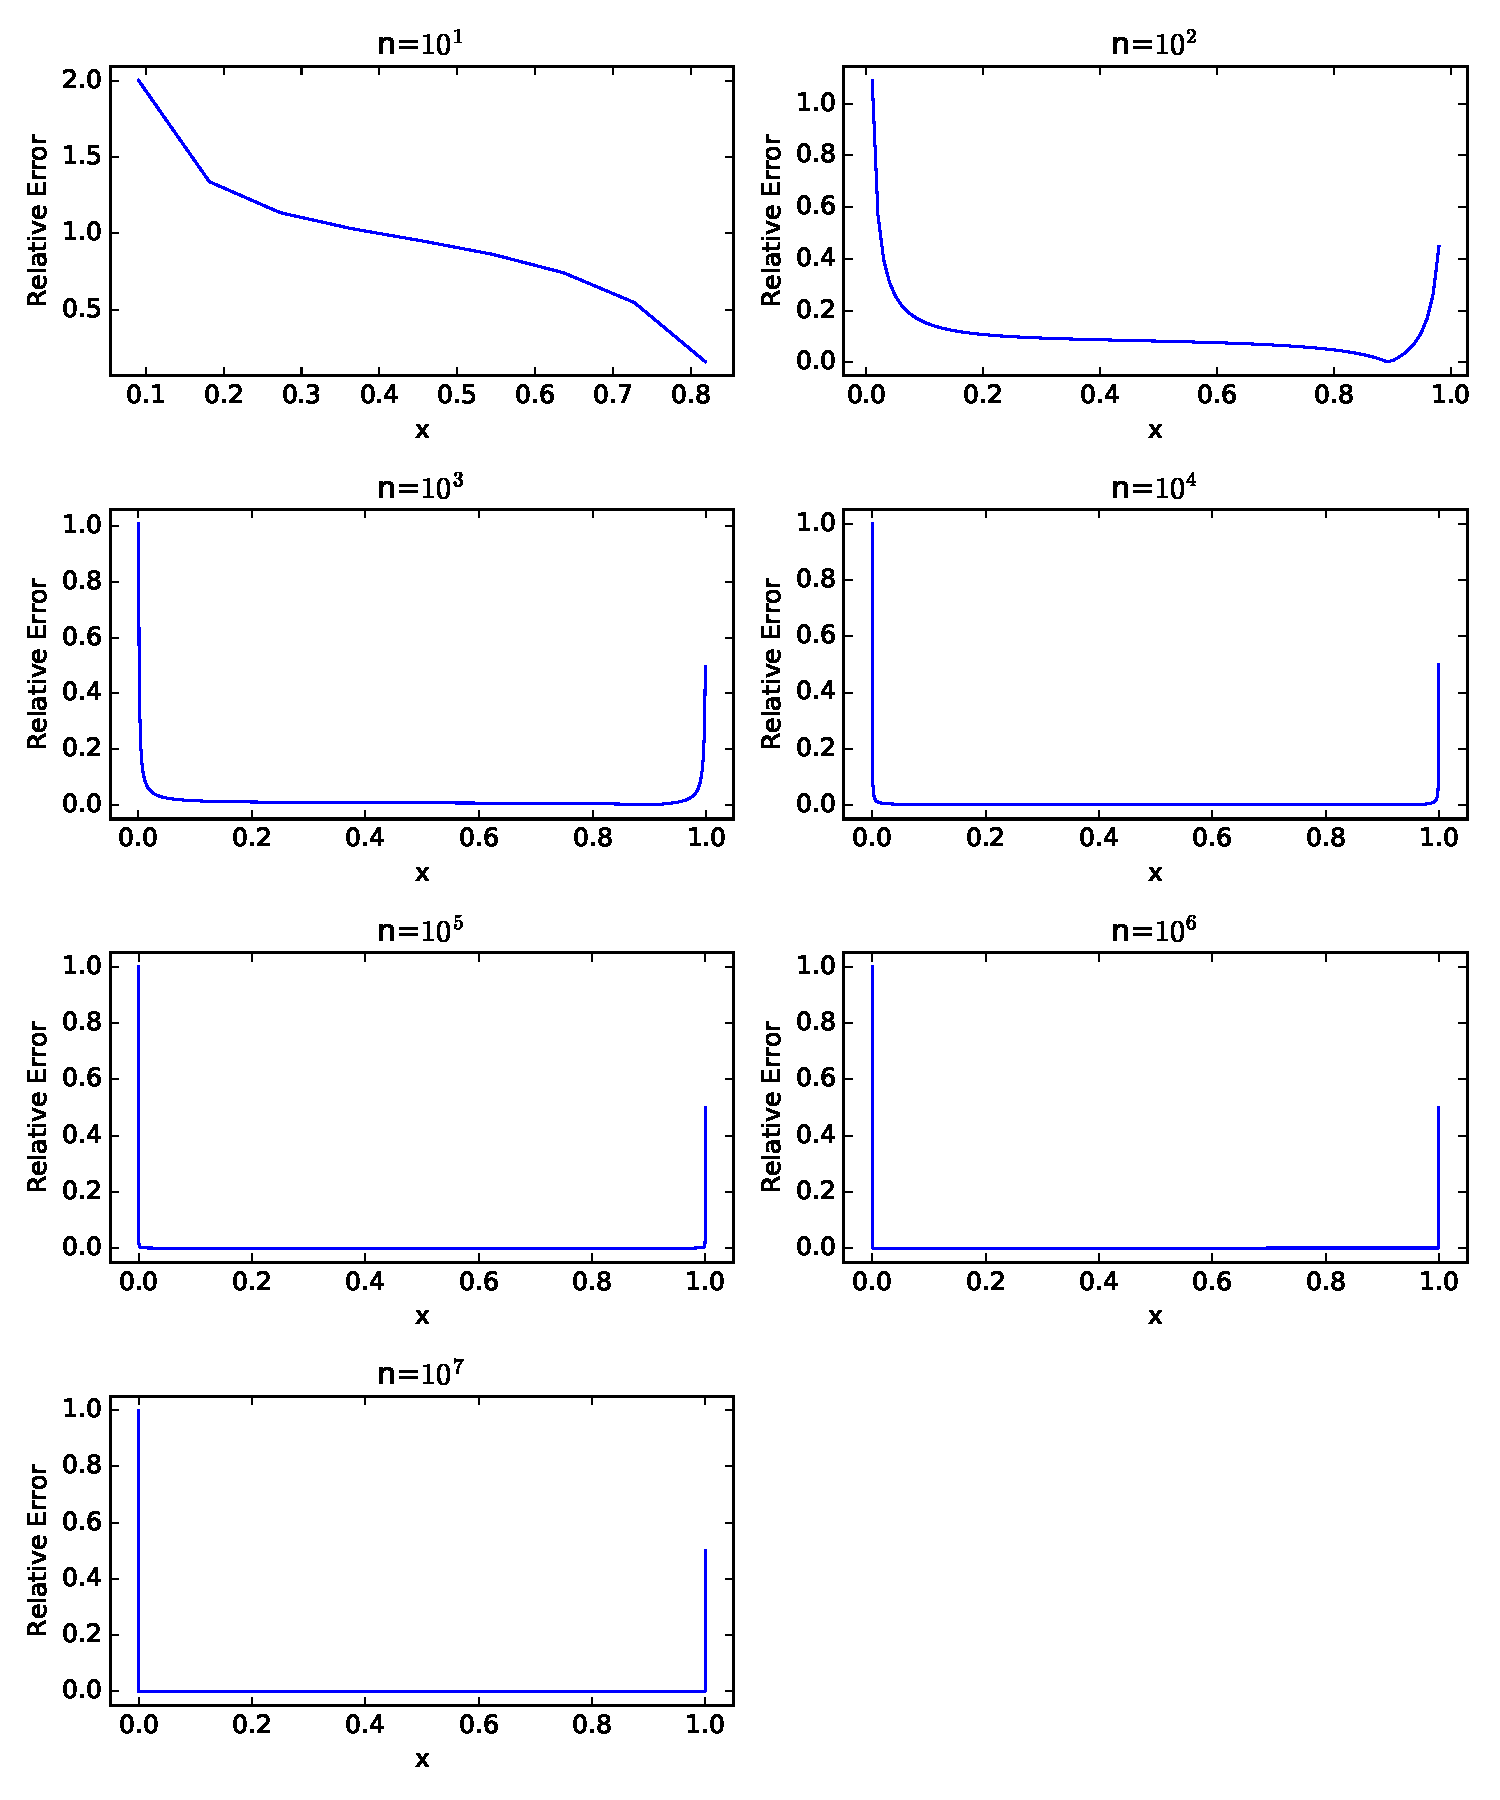
\includegraphics[width=\linewidth]{fig/rel_error.pdf}
    \caption{Relative error of the numerical solution obtained with the generic tridiagonal solver.}
    \label{fig:error}
\end{figure}

The maximum value of the relative error for each step length $h$ is displayed in table \ref{tab:error} and it seems to approach 1, with the logarithm approaching zero. Obviously, both the nominator and denominator in equation \ref{eq:error} approach zero as ${x_i}$ approaches ${x_0}$, but these results may indicate that they approach zero at different speeds.

\begin{table}[h]
\centering
\begin{tabular}{r|r|r}
Step size (h) & Max relative error($\epsilon$) & Max $log(\epsilon)$\\
\hline
$9 \times 10^{-2}$ & $2.00329251$ & $6.95 \times 10^{-1}$\\
$1 \times 10^{-2}$ & $1.09015546$ & $8.63 \times 10^{-2}$\\
$1 \times 10^{-3}$ & $1.00890166$ & $8.86 \times 10^{-3}$\\
$1 \times 10^{-4}$ & $1.00088902$ & $8.89 \times 10^{-4}$\\
$1 \times 10^{-5}$ & $1.00008889$ & $8.89 \times 10^{-5}$\\
$1 \times 10^{-6}$ & $1.00000923$ & $9.23 \times 10^{-6}$\\
$1 \times 10^{-7}$ & $1.00000307$ & $3.07 \times 10^{-6}$\\
\hline
\end{tabular}
\caption{Maximum relative error for each step length using the generic tridiagonal solver.}
\label{tab:error}
\end{table}



\subsection{Execution time and memory consumption}

The execution times of the different algorithms measured using the C++ function \texttt{std::clock()} are listed in table \ref{tab:times}. As expected the fastest algorithm is the custom made solver, followed by the generic tridiagonal solver. By the number of floating point operations the custom made algorithm was expected to be twice as fast as the generic tridiagonal solver, but in general that is not the case. The method used for timing is probably not suited for very fast algorithms and running the program multiple times yields different results, but in general the custom made algorithm is the fastest. Also, the implementations can consist of operations other than floating point operations, even though these often are very fast. The LU-decomposition, however, is visibly slower even for small $n$, which is expected.  The numbers indicate that the execution time of the LU-decomposition scale by a factor of $n^2$ faster than the other algorithms. Due to the rapidly increasing execution time and memory consumption the LU-decomposition solver is not tested for values of $n>1000$.

\begin{table}[h]
\centering
\begin{tabular}{r|r|r|r|r|r}
n & Generic & Custom & G/C & LUD & LUD/C \\
\hline
$10^{1}$ & $1.40 \times 10^{-5}$s & $3.00 \times 10^{-6}$s & $4.67$ & $1.90 \times 10^{-5}$s & $6.33$ \\
$10^{2}$ & $1.40 \times 10^{-5}$s & $1.20 \times 10^{-5}$s & $1.17$ & $7.39 \times 10^{-3}$s & $6.16 \times 10^{2}$ \\
$10^{3}$ & $5.00 \times 10^{-5}$s & $4.10 \times 10^{-5}$s & $1.22$ & $1.18$s & $2.88 \times 10^{4}$ \\
$10^{4}$ & $2.94 \times 10^{-4}$s & $2.86 \times 10^{-4}$s & $1.03$s & & \\
$10^{5}$ & $3.02 \times 10^{-3}$s & $2.55 \times 10^{-3}$s & $1.18$s & & \\
$10^{6}$ & $2.82 \times 10^{-2}$s & $2.62 \times 10^{-2}$s & $1.08$s & & \\
$10^{7}$ & $2.80 \times 10^{-1}$s & $2.55 \times 10^{-1}$s & $1.10$s & & \\
\hline
\end{tabular}
\caption{Execution times for the different algorithms and their ratio.}
\label{tab:times}
\end{table}

The generic and tridiagonal solver only uses arrays and the memory consumption therefore scales as $\mathcal{O}(n)$ with each number occupying 64bits, or 8bytes. The LU-decomposition however uses matrices and the memory consumption scales as $\mathcal{O}(n^2)$ and will become and issue for large values of $n$. For instance, with $n=10^5$ the matrix will require around 80GB of memory, while one array only requires about 0.8MB, where the implementation requires 4-5 such arrays for the generic tridiagonal solver. The custom solver requires even less.


\section{Conclusions}
\label{sec:conclusions}
The execution time of the LU-decomposition method is obviously a lot longer than the execution time of the tridiagonal solvers. When the matrix $\bm{A}$ is sparse a lot of the floating point operations in LU-decomposition is multiplication by zero, and the execution time can be reduced significantly by exploiting this knowledge as is done with the tridiagonal solvers. 

The approximation to the second order derivative is reasonable for smaller values of $h$, for instance with $n=10^4$. But the relative error becomes large near the boundary conditions because the analytical solution is approaching zero.  


\clearpage
\begin{appendices}
\section{Gauss elimination}
\label{app:gauss}

Gauss elimination of the equation system $\bm{A}\bm{v} = h^2\bm{f}$, where $a_{ij}$ is the matrix element of matrix $\bm{A}$ at row $i$ and column $j$ and $R_i$ is row number $i$.

\begin{flalign*}
&
\begin{bmatrix}
b_1    & c_1    & 0       & \cdots  & \cdots  & \cdots  & 0      \\
a_2    & b_2    & c_2     & 0       & \cdots  & \cdots  & 0      \\
0      & a_3    & b_3     & c_3     & 0       & \cdots  & 0      \\
\vdots & \vdots & \ddots  & \ddots  & \ddots  & \vdots  & \vdots \\
\vdots & \vdots & \vdots  & \ddots  & \ddots  & \ddots  & \vdots \\
0      & \cdots & \cdots  & 0       &a_{n-1} & b_{n-1} & c_{n-1} \\
0      & \cdots & \cdots  & \cdots  & 0       & a_n     & b_n    \\
\end{bmatrix}
\begin{bmatrix}
v_1 \\
v_2 \\
v_3 \\
\vdots \\
\vdots \\
v_{n-1} \\
v_n \\
\end{bmatrix}
= h^2
\begin{bmatrix}
f_1 \\
f_2 \\
f_3 \\
\vdots \\
\vdots \\
f_{n-1} \\
f_n \\
\end{bmatrix}
\\
& \text{Set $b_1=d_1$, $f_1=w_1$ and apply $R_2 = R_2 - R_1*a_{j1}/a_{11}$.} \\
&
\begin{bmatrix}
d_1    & c_1    & 0       & \cdots  & \cdots  & \cdots  & 0      \\
0      & b_2 - \frac{a_2c_1}{d_1} & c_2 - \frac{a_2*0}{b_1}   & 0       & \cdots  & \cdots  & 0      \\
0      & a_3    & b_3     & c_3     & 0       & \cdots  & 0      \\
\vdots & \vdots & \ddots  & \ddots  & \ddots  & \vdots  & \vdots \\
\vdots & \vdots & \vdots  & \ddots  & \ddots  & \ddots  & \vdots \\
0      & \cdots & \cdots  & 0       &a_{n-1} & b_{n-1} & c_{n-1} \\
0      & \cdots & \cdots  & \cdots  & 0       & a_n     & b_n    \\
\end{bmatrix}
\begin{bmatrix}
v_1 \\
v_2 \\
v_3 \\
\vdots \\
\vdots \\
v_{n-1} \\
v_n \\
\end{bmatrix}
= h^2
\begin{bmatrix}
w_1 \\
f_2 - \frac{a_2w_1}{d_1} \\
f_3 \\
\vdots \\
\vdots \\
f_{n-1} \\
f_n \\
\end{bmatrix}
\\
& \text{Set $d_2=b_2 - a_2c_1/d_1$, $w_2=f_2 - a_2w_1/d_1$ and apply $R_3 = R_3 - R_2*a_{j2}/a_{22}$.} \\
&
\begin{bmatrix}
d_1    & c_1    & 0       & \cdots  & \cdots  & \cdots  & 0      \\
0      & d_2    & c_2     & 0       & \cdots  & \cdots  & 0      \\
0      & 0      & b_3 - \frac{a_3c_2}{d_2}     & c_3 - \frac{a_3*0}{d_2}     & 0       & \cdots  & 0      \\
\vdots & \vdots & \ddots  & \ddots  & \ddots  & \vdots  & \vdots \\
\vdots & \vdots & \vdots  & \ddots  & \ddots  & \ddots  & \vdots \\
0      & \cdots & \cdots  & 0       &a_{n-1} & b_{n-1} & c_{n-1} \\
0      & \cdots & \cdots  & \cdots  & 0       & a_n     & b_n    \\
\end{bmatrix}
\begin{bmatrix}
v_1 \\
v_2 \\
v_3 \\
\vdots \\
\vdots \\
v_{n-1} \\
v_n \\
\end{bmatrix}
= h^2
\begin{bmatrix}
w_1 \\
w_2 \\
f_3 - \frac{a_3w_2}{d_1}\\
\vdots \\
\vdots \\
f_{n-1} \\
f_n \\
\end{bmatrix}
\\
& \text{Continuing this process for every row finally yields } \\
&
\begin{bmatrix}
d_1    & c_1    & 0       & \cdots  & \cdots  & \cdots  & 0      \\
0      & d_2    & c_2     & 0       & \cdots  & \cdots  & 0      \\
0      & 0      & d_3     & c_3     & 0       & \cdots  & 0      \\
\vdots & \vdots & \ddots  & \ddots  & \ddots  & \vdots  & \vdots \\
\vdots & \vdots & \vdots  & \ddots  & \ddots  & \ddots  & \vdots \\
\vdots & \cdots & \cdots  & \cdots  & 0       & d_{n-1} & c_{n-1} \\
0      & \cdots & \cdots  & \cdots  & \cdots  & 0     & d_n    \\
\end{bmatrix}
\begin{bmatrix}
v_1 \\
v_2 \\
v_3 \\
\vdots \\
\vdots \\
v_{n-1} \\
v_n \\
\end{bmatrix}
= h^2
\begin{bmatrix}
w_1 \\
w_2 \\
w_3\\
\vdots \\
\vdots \\
w_{n-1} \\
w_n \\
\end{bmatrix}
\end{flalign*}

With $d_i = b_i - a_ic_{i-1}/d_{i-1}$ and $w_i = f_i - a_iw_{i-1}/d_{i-1}$.
\clearpage
\section{LU-decomposition and backward substitution flops}
\label{app:lud}
Finding the LU-decomposition involves finding the value for $n\times n$ matrix elements (assuming a square matrix). These elements are found with the following equations, as described in \cite{lectures}:

\begin{flalign*}
u_{1j} &= a_{1j} \\
u_{ij} &= a_{ij} - \sum_{k=1}^{i-1} l_{ik}u_{kj} \quad \text{ for } i = 2,..., j-1 \\
u_{jj} &= a_{jj} - \sum_{k=1}^{j-1} l_{jk}u_{kj} \quad \text{ for } j = 1,..., n \\
l_{ij} &= \frac{1}{u_{jj}}\big(a_{ij} - \sum_{k=1}^{j-1} l_{ik}u_{kj}\big) \quad \text{ for } i > j  \\
\end{flalign*}

This shows that determining a matrix element requires at the maximum $n$ floating point operations. This means that the runtime of the LU-decomposition scales as $\mathcal{O}(n^3)$. The backward substitution is performed twice, but each application only scales as $\mathcal{O}(n^2)$ as with the tridiagonal solvers. The dominating term is therefore $\mathcal{O}(n^3)$. 

\clearpage
\section{Numerical vs Analytical solutions}
\label{app:diff_plots}
\begin{figure}[h]
    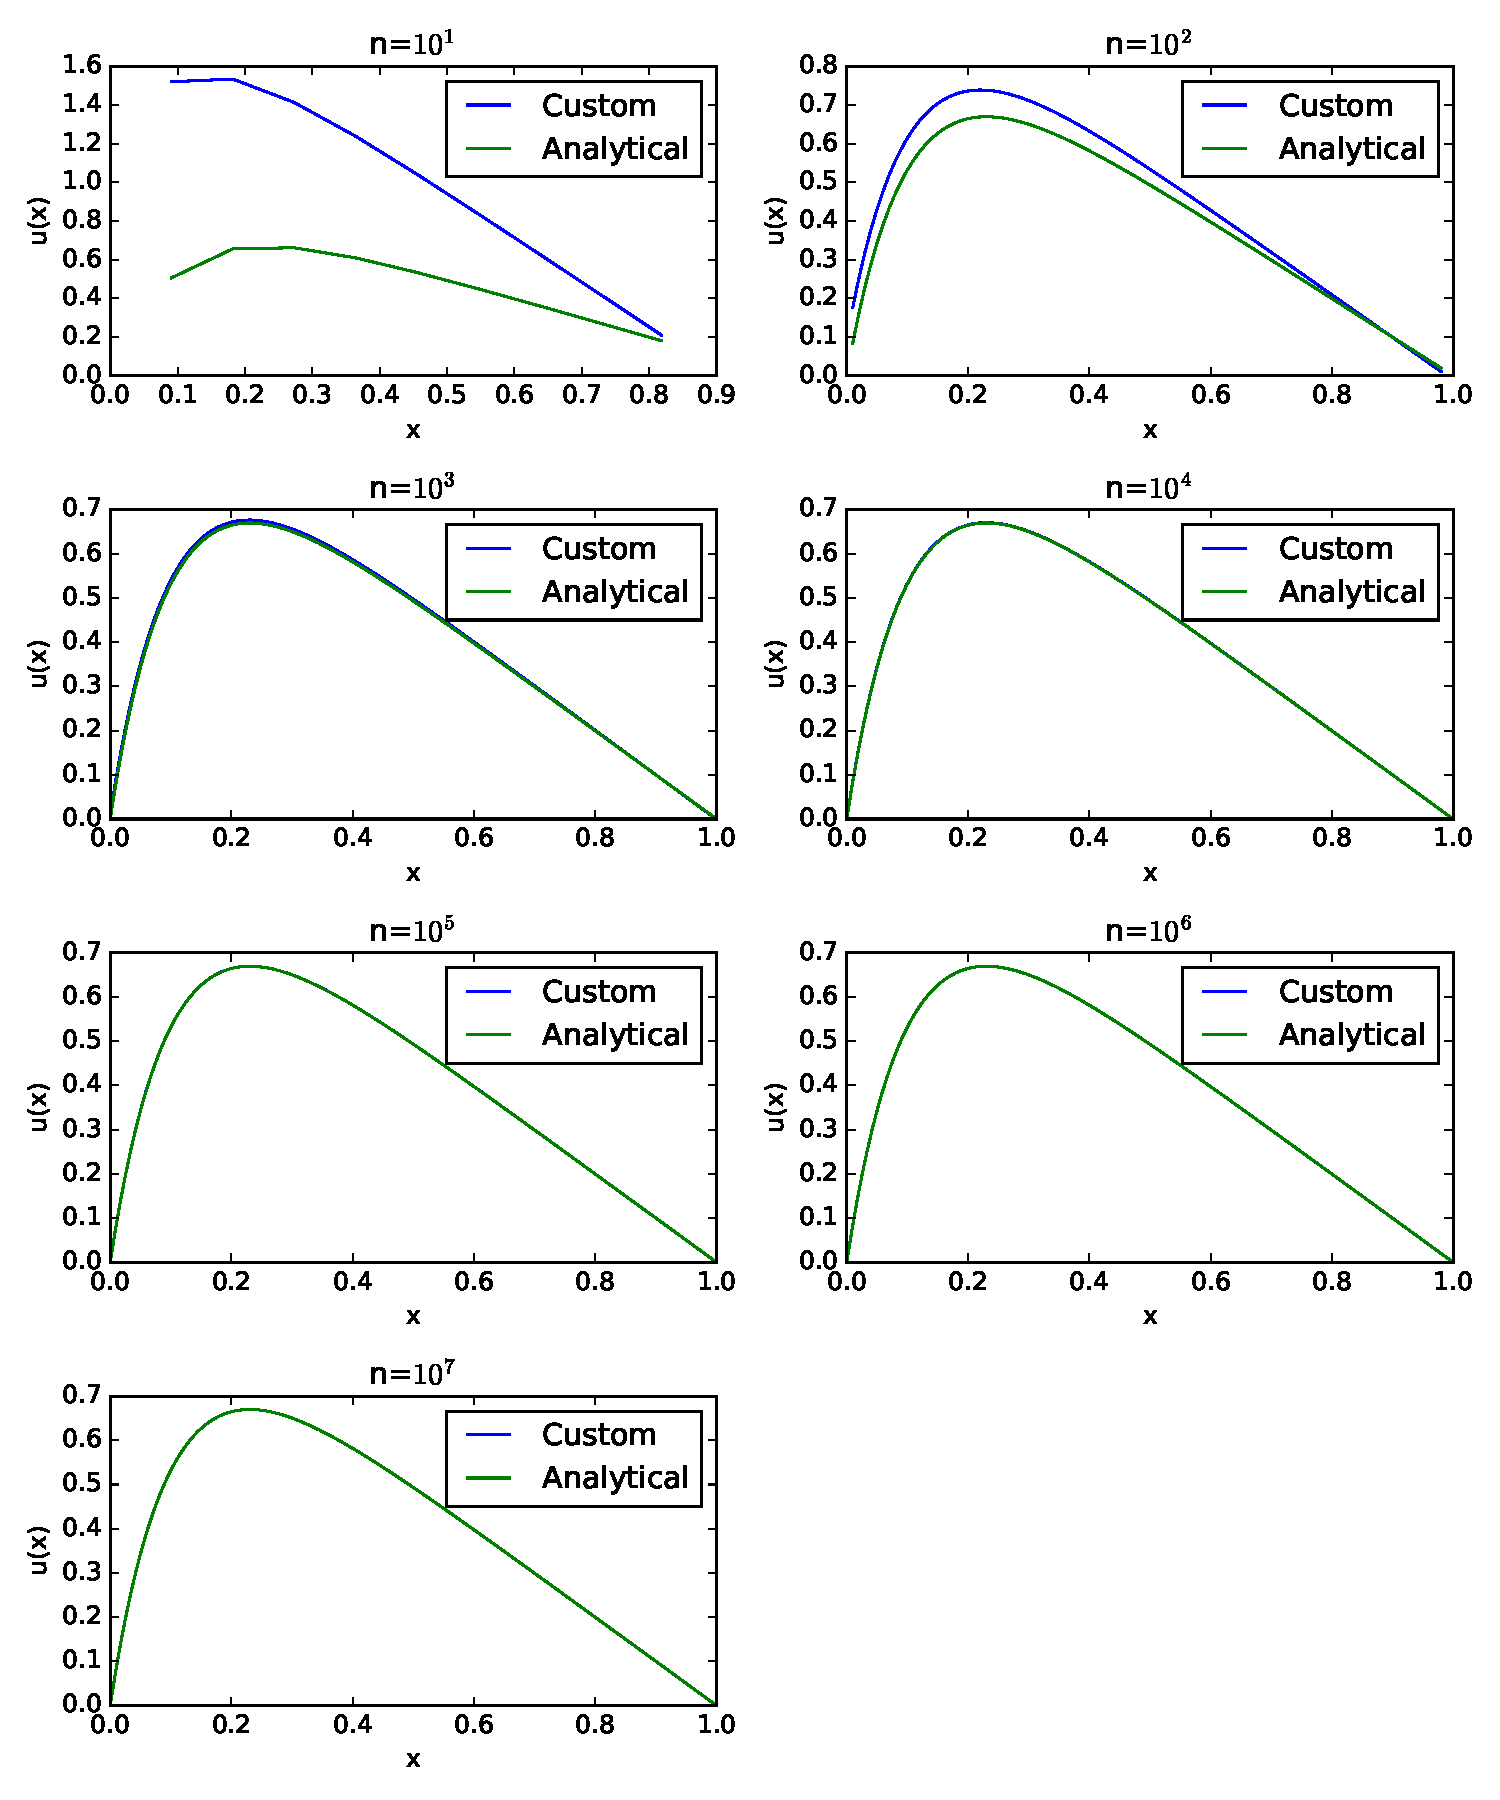
\includegraphics[width=0.9\linewidth]{fig/custom_vs_analytical.pdf}
    \caption{Numerical solution using the tridiagonal solver tailored to this specific matrix compared to the analytical solution.}
    \label{fig:s_vs_a}
\end{figure}

\begin{figure}[h]
    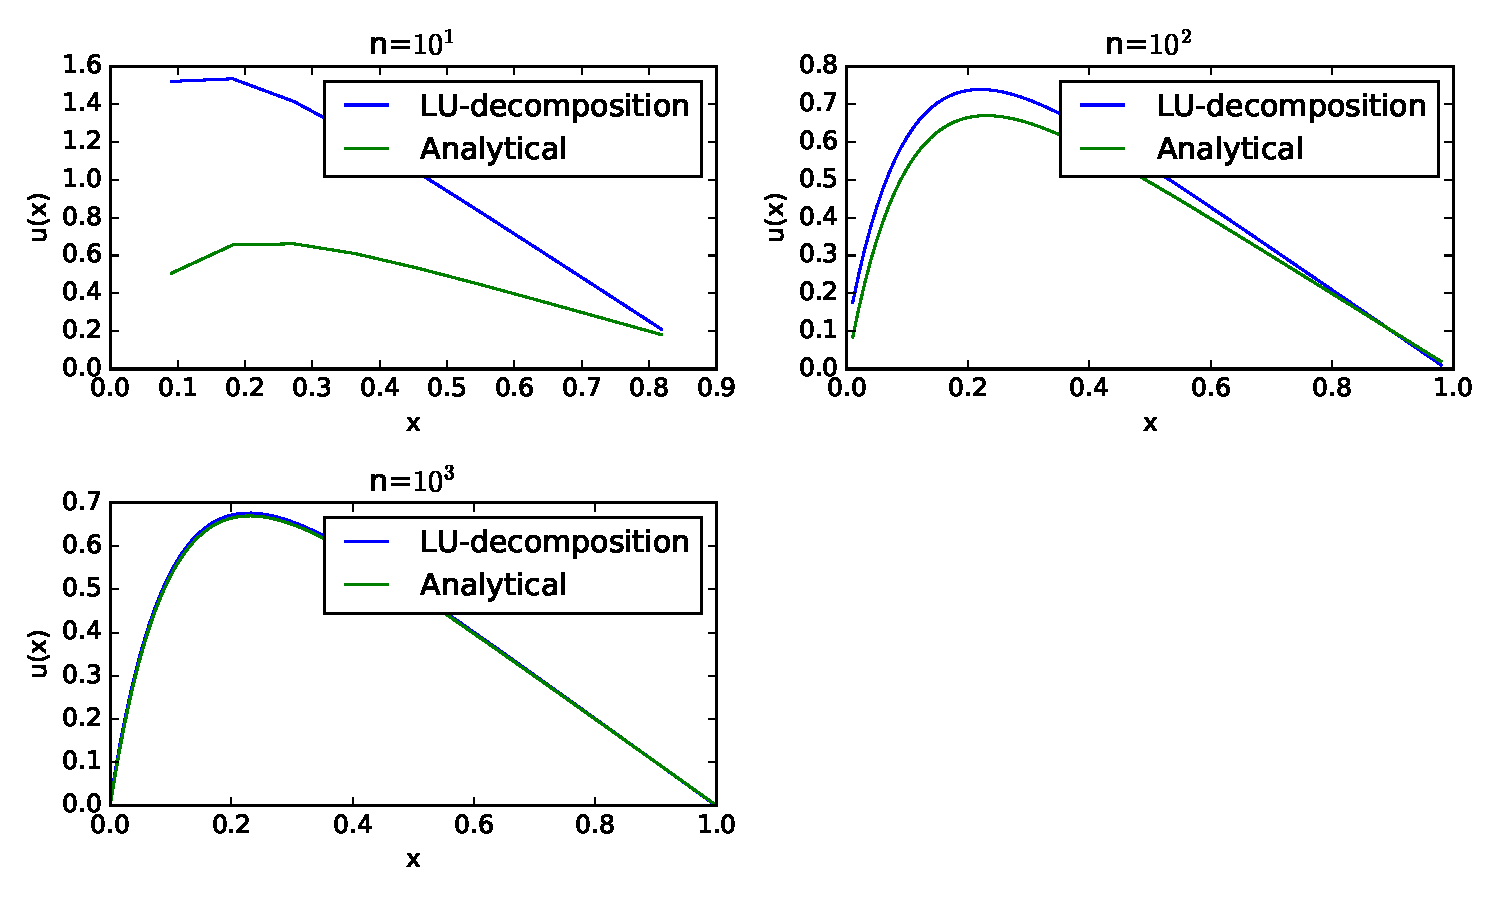
\includegraphics[width=0.9\linewidth]{fig/lud_vs_analytical.pdf}
    \caption{Numerical solution using the LU-decomposition and backward substitution compared to the analytical solution.}
    \label{fig:lud_vs_a}
\end{figure}


\end{appendices}


\clearpage

\begin{thebibliography}{1}

\bibitem{lectures} Hjort-Jensen, M., 2015. Computational physics. Available at https://github.com/CompPhysics/ComputationalPhysics/
\end{thebibliography}
\end{document}
